\documentclass[11pt,a4paper]{article}

\usepackage{fullpage}
\usepackage{rotating}
\usepackage{amsmath, amssymb, amsthm}
%\usepackage{mathpartir}
\usepackage{tikz}
\usepackage{verbatim}
\usepackage{url}
\usepackage{enumitem}
\usepackage{accents}

\usepackage{listings}
\usepackage{color}

\definecolor{dkgreen}{rgb}{0,0.6,0}
\definecolor{gray}{rgb}{0.5,0.5,0.5}
\definecolor{mauve}{rgb}{0.58,0,0.82}

\lstset{frame=tb,
  language=Java,
  aboveskip=3mm,
  belowskip=3mm,
  showstringspaces=false,
  columns=flexible,
  basicstyle={\small\ttfamily},
  numbers=none,
  numberstyle=\tiny\color{gray},
  keywordstyle=\color{blue},
  commentstyle=\color{dkgreen},
  stringstyle=\color{mauve},
  breaklines=true,
  breakatwhitespace=true,
  tabsize=3
}

\usetikzlibrary{trees}

\begin{document}
\title{WACC Compiler Group Project}
\author{Elyas Addo, Florian Emile, Elliot Greenwood, Jonathan King}

\maketitle

\section{The Product}
\label{sec:The Product}

\subsection{Functionality}
\label{sub:Functionality}

The front end for our compiler demonstrated the correct functionality for all test files. We were allowing valid WACC files through to the code generation stage, and preventing any files with errors through. After performing the lexical, syntactic and semantic analysis on any invalid input WACC files, the compiler would output useful errors; the line and column number followed by a message outlining the error pitching snippets of their code for context against the expected value.

For the code generation milestone our compiler was functionally correct a large majority of our test cases. The only exceptions are cases in which where there is a pair or array that is freed more than once (without being reinitilised). In these cases we should be throwing a runtime exception and exiting with status code 134; however we throw a null reference exception is thrown instead.

\subsection{Extensibilty}
\label{subs:Extensibilty}

The neatness of our design was always kept in mind whilst implementing our compiler. We wanted to make sure that our code could easily be adapted in the future, perhaps with additional languages features or compiling into a different language.

As we knew we would have to do an extension, the ability to easily change the compiler was very important. To facilitate the ability to add any new features we used the visitor pattern frequently. Due to the fact all of our visit functions only knew about their context, for each new language feature it was a simple case of adding a new visit function. There were a few exceptions when we had to check for a null value of a child node in our syntax tree.

One aspect we overlooked was creating our own tree structure to represent the program. We used the parse tree provided by ANTLR which meant that if we were to replace ANTLR for a similar, but perhaps more up-to-date, tool we would have to rewrite a lot of our code base. Building an Abstract Syntax Tree (AST) of our own would mean that our methods for code generation could remain intact. We would simply need to create a class to convert from the new tool-created tree to our own AST. Having control over the tree and information stored in each node would also dramatically help within visitor methods. It could remove a lot of checks on the fields in nodes as they would provide all and only the relevant information related to a particular part of the code. 

A good deal of thought was put into the possibility of changing the output language. In a few years ARM11 may not be desirable; by extracting all the ARM11 specific code into it's own package, changing the output language would simply involve swapping that package for, say, a x86 package. Our code would not change as the instruction factory would simply return x86 instructions as opposed to ARM11 instructions.

\section{The Project Management}
\label{sec:The Project Management}

\subsection{Group Structure}
\label{sub:Group Structure}

We split our group into twos, and would pair program for larger sections of feature implemenations. For smaller sections, members would work independently.

The pair programming made catching simple mistakes easier and forced us to discuss design choices, logical processes and other decisions before implementing them, leading to many fewer errors to debug. The independent work for smaller sections meant we were able to get more work done in a smaller amount of time and not have a member sat idle for trivial implementations.

\subsection{Use of Project Management Tools}
\label{sub:Use of Project Management Tools}

To help organise the team we used a few project management tools and continuous integration platforms.

\subsubsection{Maven}
\label{subs:Maven}

We used Maven to structure our project. Using Maven meant we didn't have to take care of dependencies, such as ANTLR, the make process was also simplified as using the command \texttt{mvn package} would generate the ANTLR java files, test our code using the unit tests we had created and package our code, including the dependencies, into a .jar file.


\subsubsection{Git and Github}
\label{subs:Git and Github}

We used Git and Github as our chosen version control. We utilised branches to keep features and sub features seperate, then use pull requests to merge all of our features together. Below is a diagram showing the main branches for our project.

\tikzstyle{every node}=[draw=black,thick,anchor=west]
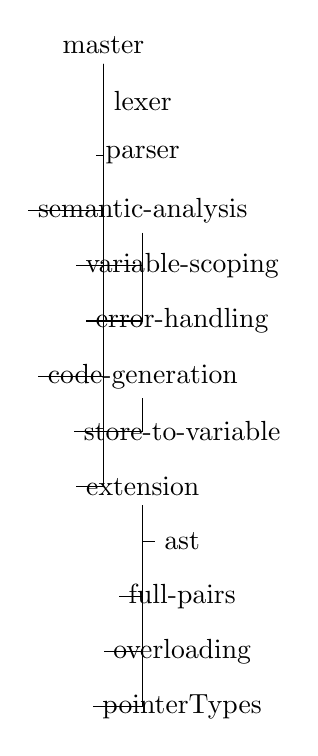
\begin{tikzpicture}[%
  grow via three points={one child at (0.5,-0.7) and
  two children at (0.5,-0.7) and (0.5,-1.4)},
  edge from parent path={(\tikzparentnode.south) |- (\tikzchildnode.west)}]

  \node {master}
    child { node {lexer}}
    child { node {parser}}
    child { node {semantic-analysis}
      child { node {variable-scoping}}
      child { node {error-handling}}
    }
    child [missing] {}
    child [missing] {}
    child { node {code-generation}
      child { node {store-to-variable}}
    }
    child [missing] {}
    child { node {extension}
      child { node {ast}}
      child { node {full-pairs}}
      child { node {overloading}}
      child { node {pointerTypes}}
    };
\end{tikzpicture}

Github provided us with Issues which we used to keep track of current bugs and enhancements we wanted to implement. It also gave us the option to assign that issue to a member of our team.

Our git commit messages on the whole were quite short and vague, though the style of our messages were on the correct path. Where possible we would style our commit messages to include the people who were working on the commit, an instruction that would tell the reader what the commit should do (i.e. Implement x instead of Implemented x).

\subsubsection{Travis}
\label{subs:Travis}
We used Travis, a continuous intergration tool, that would test our code on every push and pull request. Travis intergrates with Github and meant we would never merge a pull request in the event of our commit failing the unit tests. [How this helped]

\subsection{Slack}
\label{sub:Slack}
Our communication platform of choice was Slack, we liked the features is boasted such as channels, intergrations and snippets, which can be non-existent to contrived in other apps such as Facebook and Email.

Channels meant we could have a seperate section for each milestone, as well as a general channel for of topic conversation. This kept all of our WACC messages in one place that was not polluted by other conversations.

Integrations were really useful, the two intergrations we used the most were Github and Travis. Every time we made a commit, a new branch, an issue, assigned an issue to someone, etc. it would be automatically posted on the relevant Slack channel so everyone could read it. This stopped the need for people to ask when something had been pushed, and meant we could easily reference a certain commit. One intergration we would have liked to have used more is Wunderlist, that way we could create a centralised list of all the tasks we had todo instead of having our own lists.

Snippets were useful if we needed to send each other short pieces of code that did not warrant a commit. We would also create snippets containing the key errors produced from running tests so everyone could see what the stack trace and actual output was without us having to run the tests n times.

\subsection{What Would We Do Differently?}
\label{sub:What Would We Do Differently?}

If we were to do this lab exercise again, we would include the creation of an AST form the start. The AST could be built as soon as parsing the input file is complete. If this building process were to occur at this point in compilation, types would be created at the same time. This would remove the need for a separate visitor to create types when building the symbol table.

In terms of compiler outputs, we would like to create more user-friendly error messages. This includes changing the ANTLR error messages produced in lexical and syntactic analysis to not display a set of possible characters, but instead information on how the particular program construct should be written.
- AST
- Different method used instead of a visitor pattern creating types -> built into AST
- more detailed error messages
- Write more JUnit tests for the java classes 

\section{The Design Choices}
\label{sec:The Design Choices}

\subsection{Visitor}
\label{sub:Visitor}
[UPDATE THIS SECION IF WE FINISH THE TREE]\\
We used the visitor pattern four times in our project. We used it for our front end create types for variables to add to our symbol tables, creating the symbol tables and checking the type of expressions and statements etc. were valid according to the WACC specification. We used it in back end as well to generate the correct assembly code. We used this pattern because it gives us the flexibility to have one tree which we then can then walk over and do different tasks, otherwise each node would have to know what to do for each task and to add a knew task you would need to edit all of the node class files. This is especially undesirable as running \texttt{make} will rebuild the ANTLR files thereby removing any custom code we had added.

\subsection{Factory}
\label{sub:Factory}
To create our instructions we created a Factory to produce all the different types. This way instead of creating a class for each type of instruction we return an anonymous class that implements the interface \texttt{Instruction}. We used Java 8 lambdas to create the instructions as there is only one method \texttt{printInstruction}. This gave a clean and minimal solution to creating all of our instructions.

\subsection{Command Line Interface Seperation}
\label{sub:Command Line Interface Seperation}
We used redirection in our compile script to allow our input file to be passed in as the System.in, this means our compiler does not need to know about files it can just take the contents of the file and create an input stream,

\section{Beyond the Specification}
\label{sec:Beyond the Specification}
For our extension, we implemented language extensions. We allow function overloading: we can make functions which have the same name but a different \texttt{paramList}. We extended the WACC language with a C-style pointer type: we can now access a variable using its memory address using \texttt{*} followed by the pointer name. To get the address of a variable we created an address operator: \texttt{\&} (we need this to initialise pointers). If statements without an else case are now valid. We extended WACC language with a full typing system for pairs that does not lose type information for nested pairs.
To make sure our extensions were working properly we wrote new valid and invalid tests in WACC and created a script that notifies us if the compiler is not behaving the way it should.

If we would have had more time, we would have liked to implement some optimisations on our assembly code such as efficient register allocation and array-bound analysis. We were also quite keen on making WACC object oriented: so we would have liked to implement classes, inheritance, the advanced features of classes such as multiple-inheritance, overriding and class constructors.

\end{document}
